\documentclass[a4paper, 12pt]{article}%тип документа

%отступы
\usepackage[left=2cm,right=2cm,top=2cm,bottom=3cm,bindingoffset=0cm]{geometry}

%Русский язык
\usepackage[T2A]{fontenc} %кодировка
\usepackage[utf8]{inputenc} %кодировка исходного кода
\usepackage[english,russian]{babel} %локализация и переносы

%Вставка картинок
\usepackage{graphicx}
\graphicspath{{pictures/}}
\DeclareGraphicsExtensions{.pdf,.png,.jpg}

%Графики
\usepackage{multirow}
\usepackage{pgfplots}
\pgfplotsset{compat=1.9}

%Римские цифры
\newcommand{\RNumb}[1]{\uppercase\expandafter{\romannumeral #1\relax}}

%Математика
\usepackage{amsmath, amsfonts, amssymb, amsthm, mathtools}

%Заголовок
\author{Богданов Александр \\
	Б05-003}
\title{\textbf{Работа 5.5.5 \\ 
		Компьютерная сцинтилляционная $\gamma$-спектрометрия}}

\begin{document}

\maketitle

\textbf{Цель работы:} в данной работе проводится исследование спектров $\gamma$-лучей от различных образцов при помощи сцинтилляционных $\gamma$-спектрометров на основе неорганического кристалла NaI(Tl) и органической сцинтиллирующей пластмассы. 

\textbf{В работе используются:} сцинтиллятор,  фотоэлектронный умножитель (ФЭУ), предусилитель импульсов,  высоковольтный блок питания ФЭУ,  блок АЦП,  компьютер для сбора данных.\\

\textbf{Теоретические положения:}\\\par

	При прохождении $\gamma$-квантов через материальную среду образуются электроны,  возникающие за счет фотоэффекта,  комптоновского рассеяния и рождения электрон-позитронных пар.  Образующиеся при этих процессах электроны испытывают большое количество неупругих соударений с молекулами и атомами среды.  Неупругие соударения могут сопровождаться как ионизацией,  так и возбуждением молекул или атомов среды.  При переходах возбужденных молекул или атомов в основное состояние, при рекомбинации электрических зарядов и т.п.  в веществе возникают кванты света различных длин волн,  присущих данному веществу. 

	Возникающее излучение должно сильно поглощаться в сцинтилляторе,  так как его энергия в точности равна энергии возбуждения атомов среды.  Чтобы избежать этого явления,  в кристаллы сцинтиллятора вводят небольшие добавки других атомов.  При этом спектр поглощения сдвигается относительно спектра испускания в сторону меньших длин волн,  и увеличивается вероятность выхода из вещества хотя бы некоторой части квантов света,  отвечающих длинноволновому краю спектра испускания.  В этом случае прохождение ионизирующей частицы через вещество будет сопровождаться световой вспышкой,  которая и может быть использована для регистрации частицы. 

	Даже при поглощении частиц с одинаковой энергией амплитуда импульса на выходе фотоприёмника сцинтилляционного детектора меняется от события к событию.  Это связано со статистическим характером процессов сбора фотонов на фотоприёмнике и последующего усиления,  с различной вероятностью доставки фотона к фотоприёмнику из разных точек сцинтиллятора и с разбросом высвечиваемого числа фотонов.  Поэтому линия на спектре размывается.  Её часто описывают гауссианом.  В данной работе используется этот метод обработки данных. \\

	Энергетическим разрешением спектрометра называется величина:
\[R_i = \dfrac{\Delta E_i}{E_i} \propto \dfrac{1}{\sqrt{E_i}}\]

\textbf{Экспериментальная установка:}\\\par

\begin{figure}[h!]
	\centering
	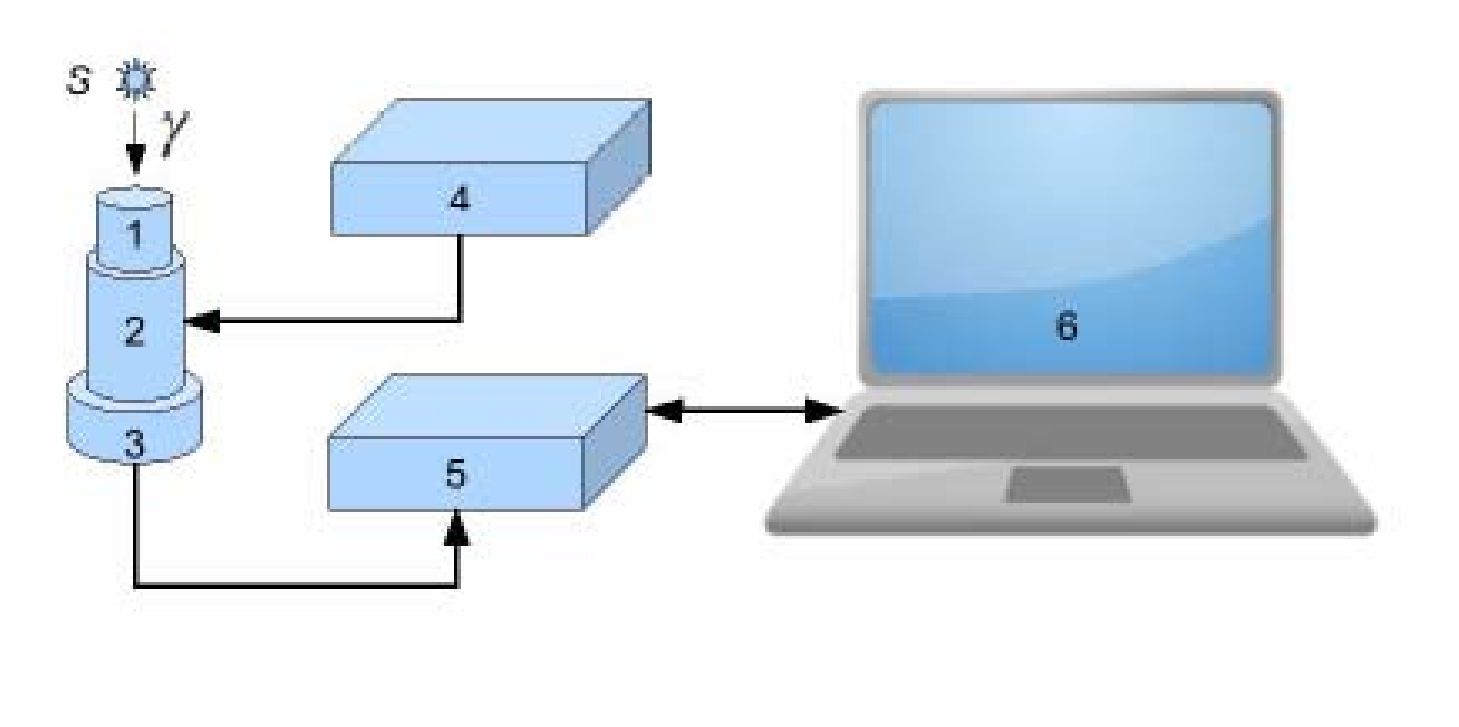
\includegraphics[scale=0.4]{Установка.PNG}
\end{figure}

\begin{enumerate}

	\item Сцинтиллятор

	\item ФЭУ
	
	\item Предусилитель импульсов
	
	\item Высоковольтный блок питания для ФЭУ
	
	\item Блок преобразования аналоговых импульсов с ФЭУ в цифровой код (АЦП)
	
	\item Компьютер для сбора данных,  их обработки и хранения\\

\end{enumerate}

\textbf{Ход работы:}\\\par

\begin{enumerate}

	\item Настроим установку.
	
	\item Убедимся,  что на полученной картине фонового спектра отсутствуют какие-либо фотопики.

	\item	 Найдем пики полного поглощения для веществ $^{22}$Na, $^{60}$Co, $^{137}$Cs, $^{152}$Eu и $^{241}$Am.  Спектр фона и спектры исследуемых веществ:
	 
	\begin{figure}[h!]
	\begin{minipage}[h]{0.47\linewidth}
		\centering
		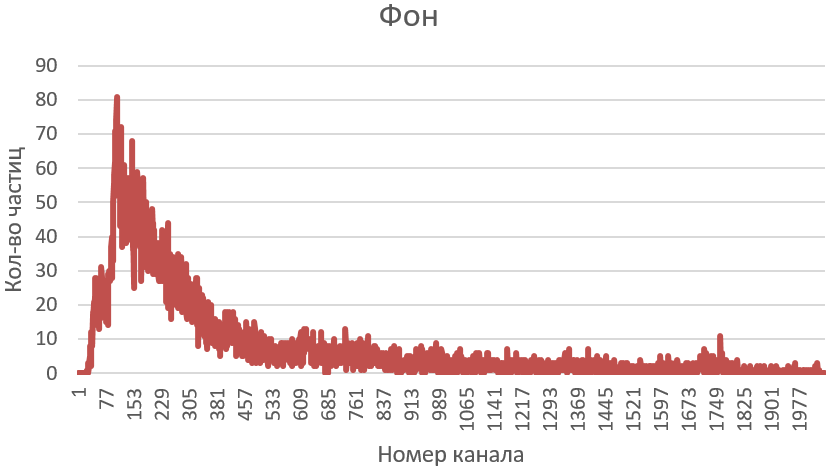
\includegraphics[scale=0.28]{fon}
	\end{minipage}
	\hfill
	\begin{minipage}[h]{0.47\linewidth}
		\centering
		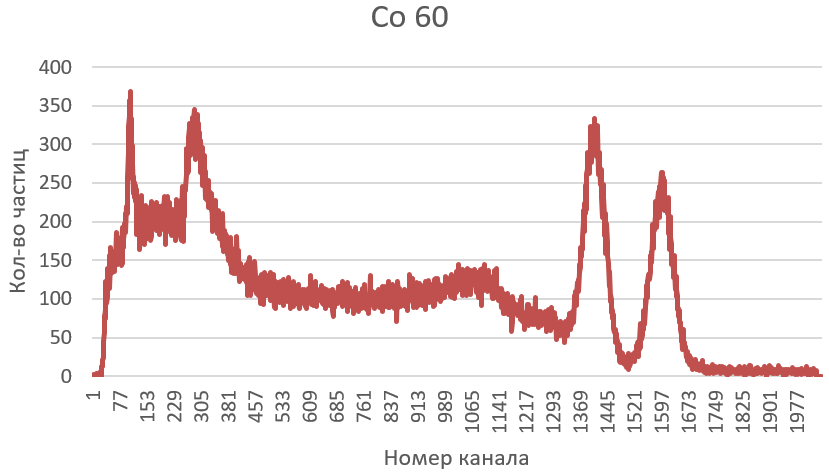
\includegraphics[scale=0.28]{Co}
	\end{minipage}
\end{figure}

\begin{figure}[h!]
	\begin{minipage}[h]{0.47\linewidth}
		\centering
		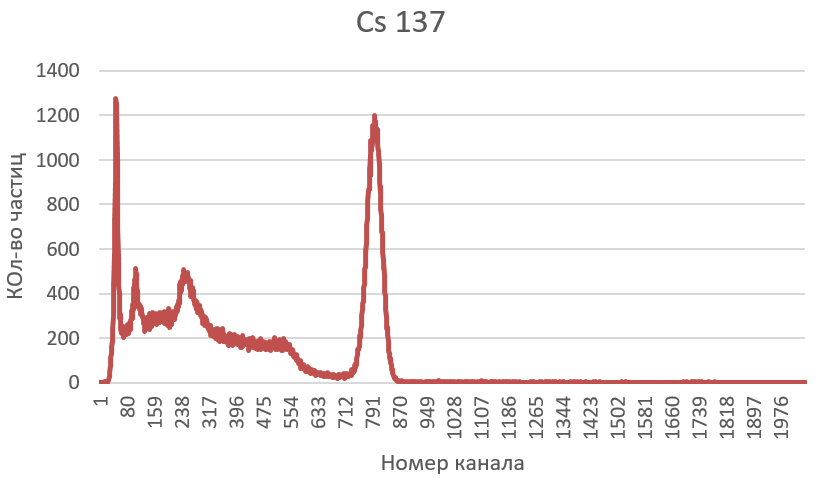
\includegraphics[scale=0.28]{Cs}
	\end{minipage}
	\hfill
	\begin{minipage}[h]{0.47\linewidth}
		\centering
		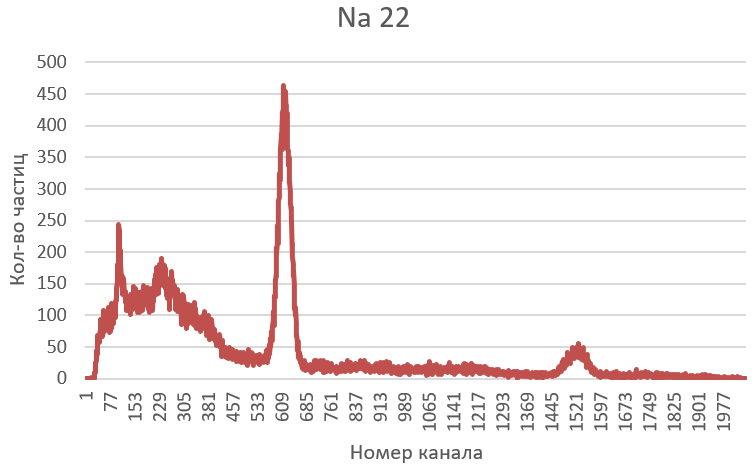
\includegraphics[scale=0.31]{Na}
	\end{minipage}
\end{figure}

\begin{figure}[h!]
	\begin{minipage}[h]{0.47\linewidth}
		\centering
		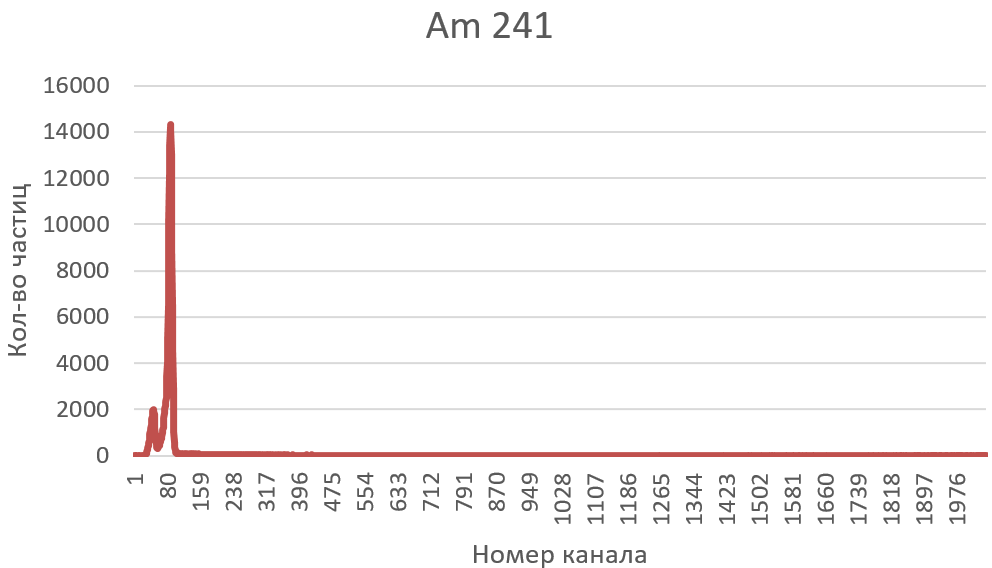
\includegraphics[scale=0.25]{Am}
	\end{minipage}
	\hfill
	\begin{minipage}[h]{0.47\linewidth}
		\centering
		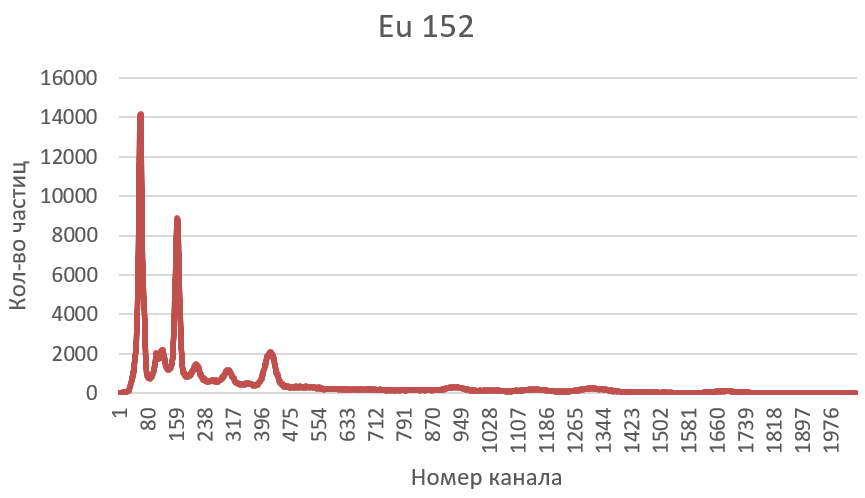
\includegraphics[scale=0.28]{Eu}
	\end{minipage}
\end{figure}

\newpage

	\item Получим на экране осциллографа устойчивое изображение импульсов с выхода ФЭУ:

\begin{figure}[h!]
	\centering
	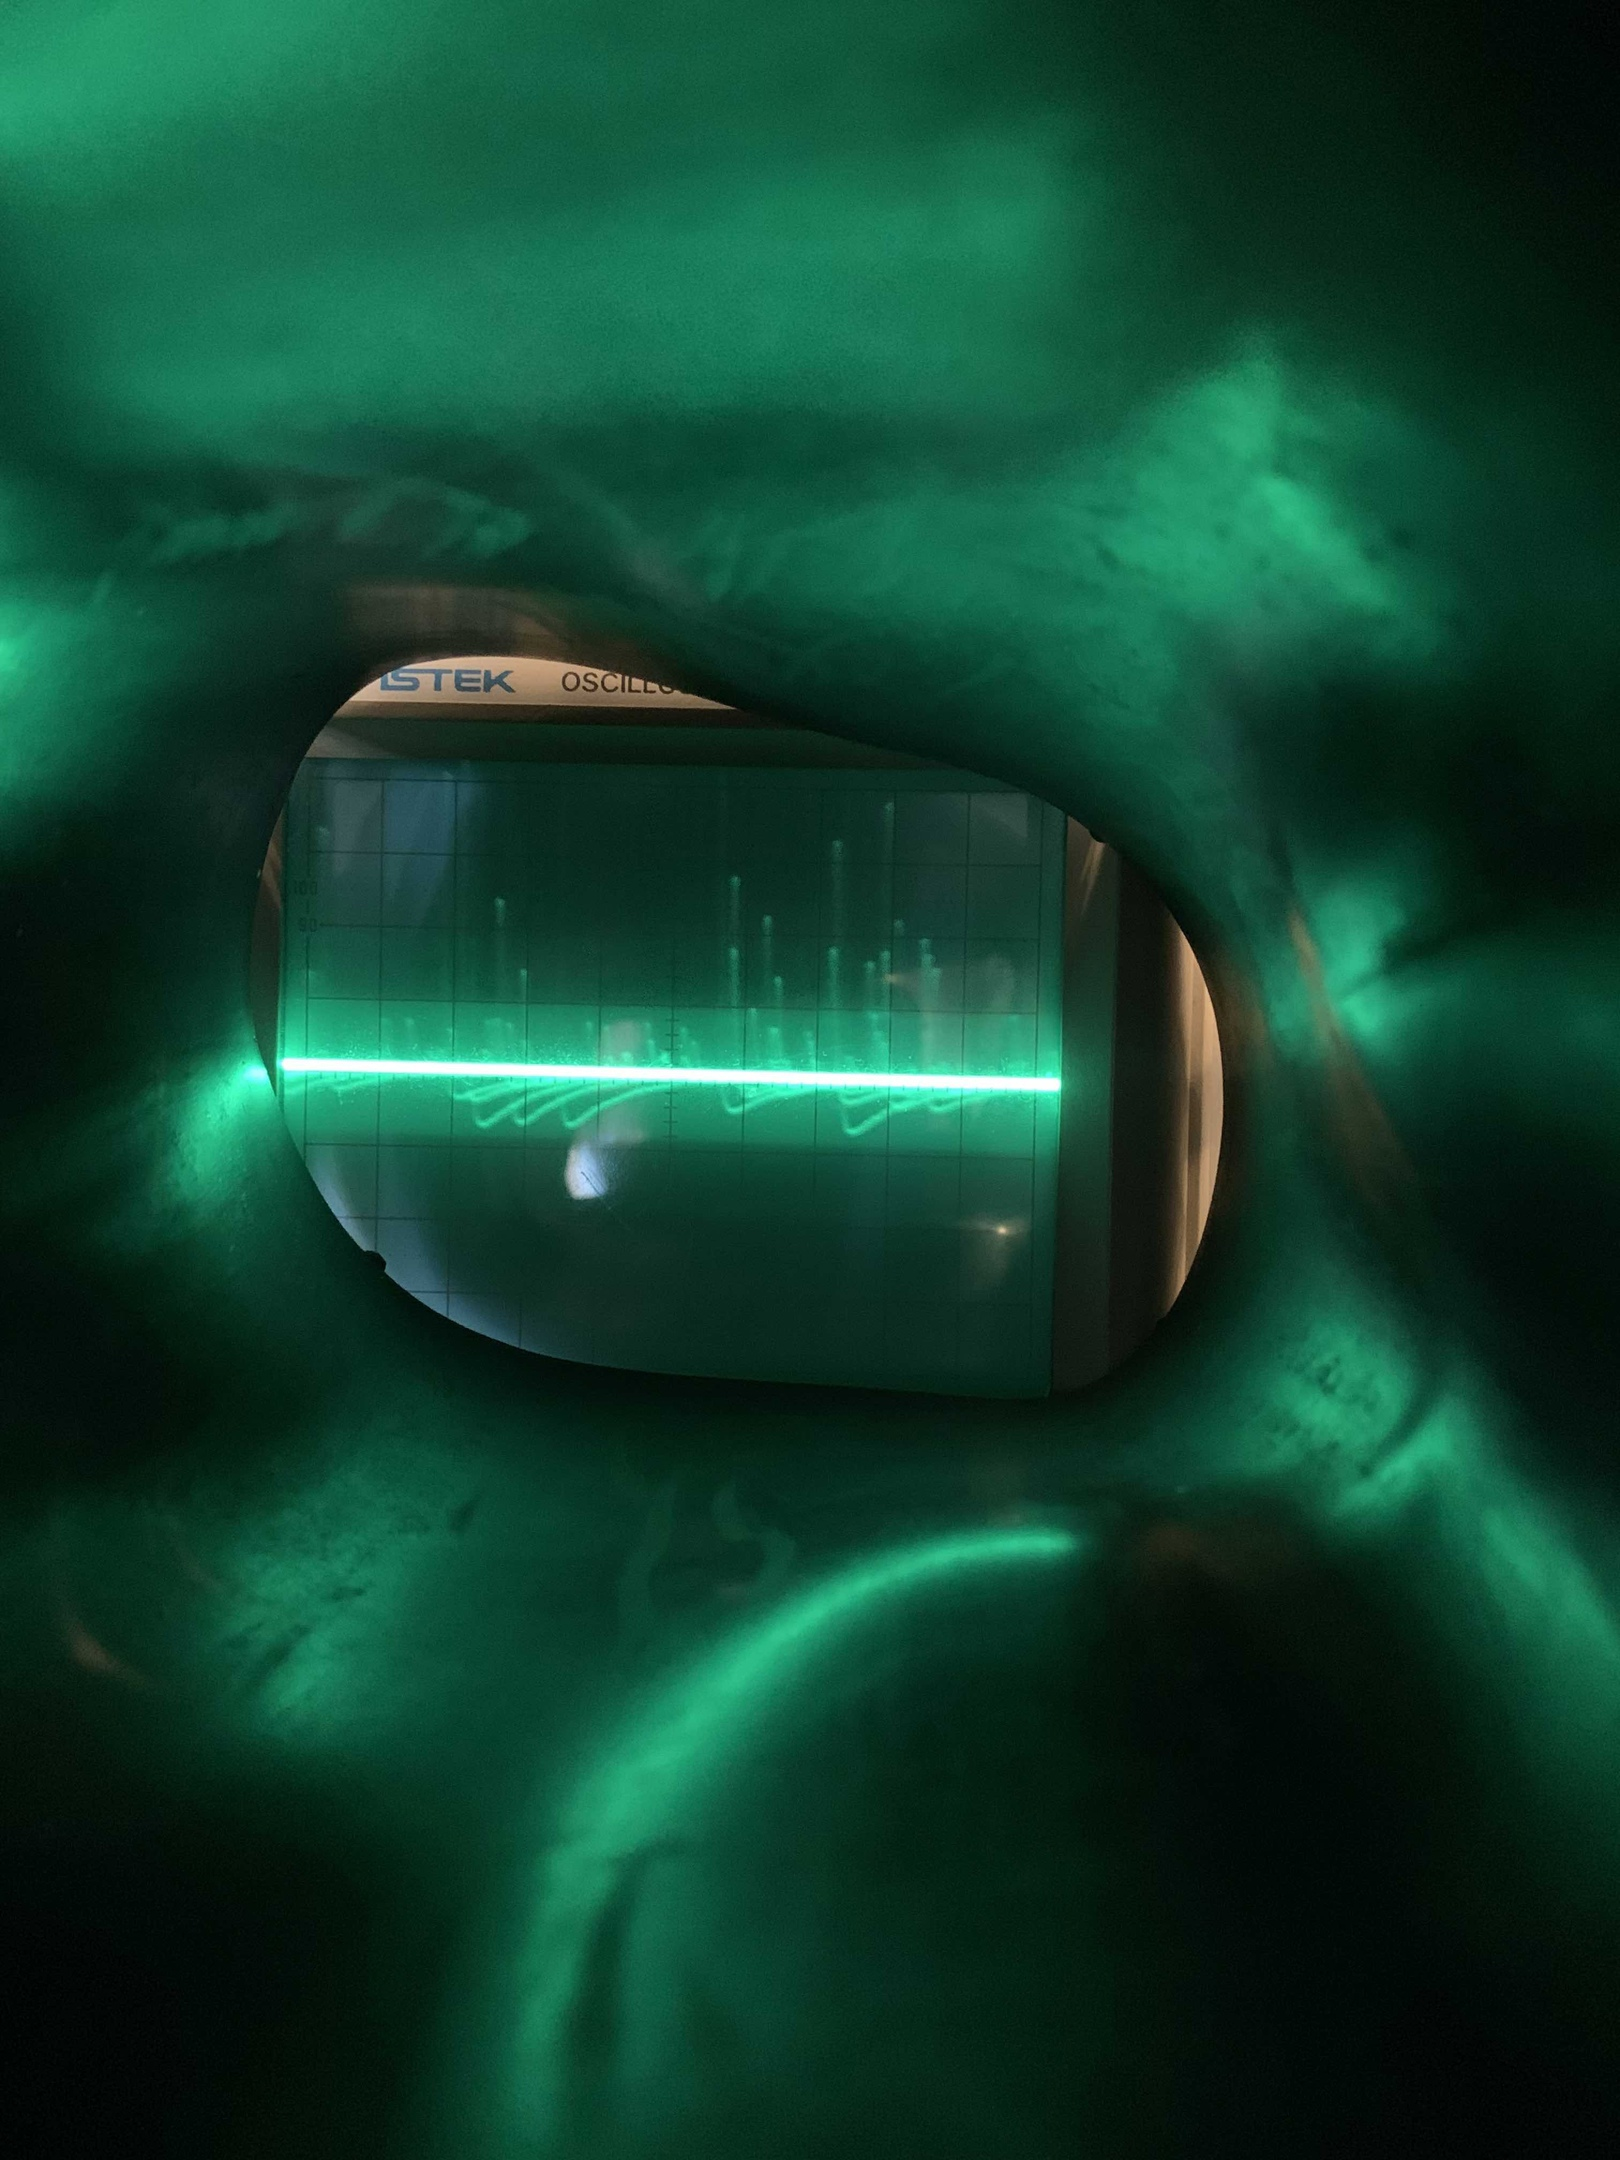
\includegraphics[scale=0.09]{Импульсы.PNG}
\end{figure}

	\item В каждом спектре определим номера каналов,  отвечающих центрам пиков полного поглощения излучения от радиоактивных источников $^{22}$Co и $^{137}$Cs.  Этим каналам присвоим табличные значения энергий и проведем линейную аппроксимацию зависимости энергии от номера канала для данного $\gamma$-спектрометра при данной геометрии измерения и настройках $\gamma$-спектрометра.  Построим калибровочный график зависимости номера канала от энергии $\gamma$-кванта:
	
\begin{figure}[h!]
	\centering
	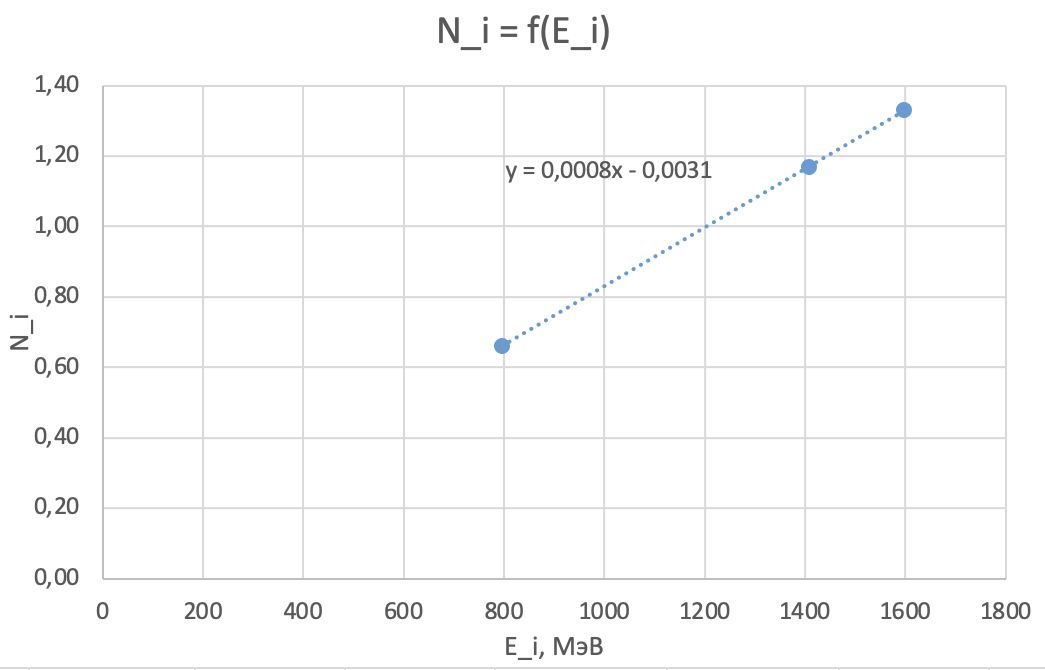
\includegraphics[scale=0.7]{График_1.PNG}
\end{figure}

	\item С помощью графика получим формулу для энергии: $ E_i = 0,008N_i - 0.0031$ МэВ.  Используя калибровочный график,  определим для всех остальных источников значения энергии пиков полного поглощения $ E_i $, их ширины на половине высоты $\Delta E_i$ и энергетическое разрешение $ R_i $:
	
\begin{figure}[h!]
	\centering
	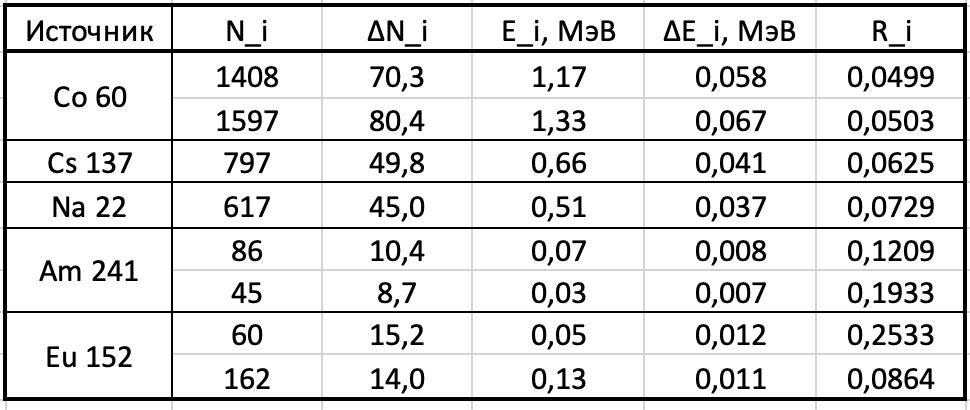
\includegraphics[scale=0.7]{Таблица_1.PNG}
\end{figure}

	\item Энергия края комптоновского поглощения для $^{22}$Na, $^{60}$Co, $^{137}$Cs:
	
\begin{figure}[h!]
	\centering
	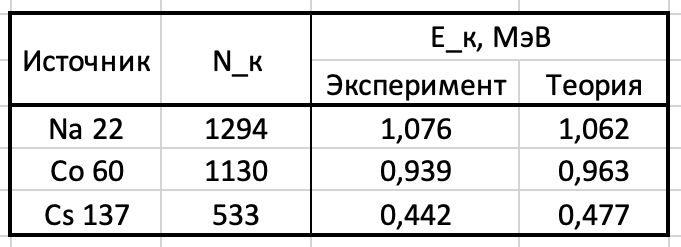
\includegraphics[scale=0.7]{Таблица_2.PNG}
\end{figure}

\newpage

	\item Построим график,  по одной оси которого отложим экспериментальные значения,  а по другой -- расчетные значения этой энергии. 
	
\begin{figure}[h!]
	\centering
	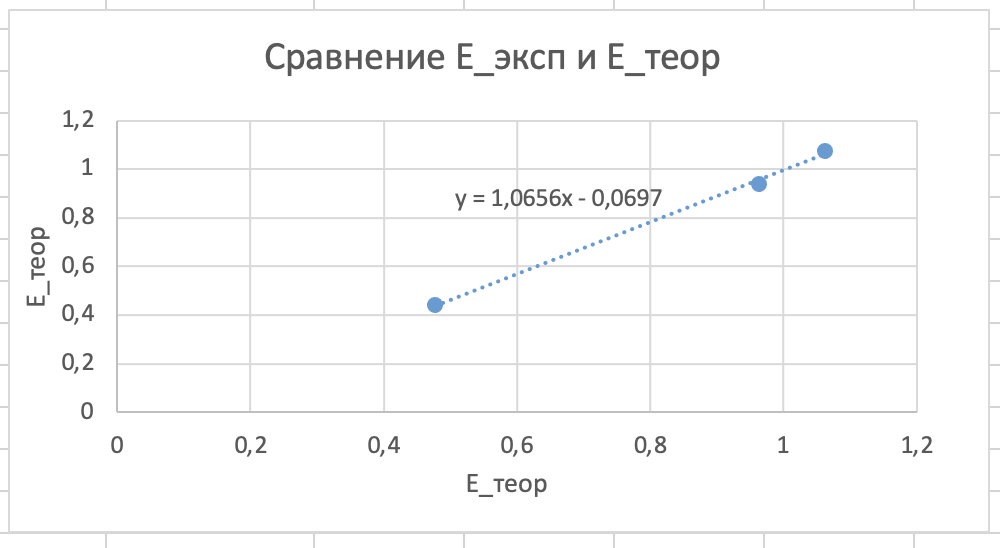
\includegraphics[scale=0.7]{График_2.PNG}
\end{figure}

	\item Для проверки зависимости $R_i = \frac{C}{\sqrt{E_i}}$ построим график $R_i^2 = f(\frac{1}{E_i})$. Значение минимальной энергии для $^{241}$Am,  из-за большой погрешности исключим.
	
\begin{figure}[h!]
	\centering
	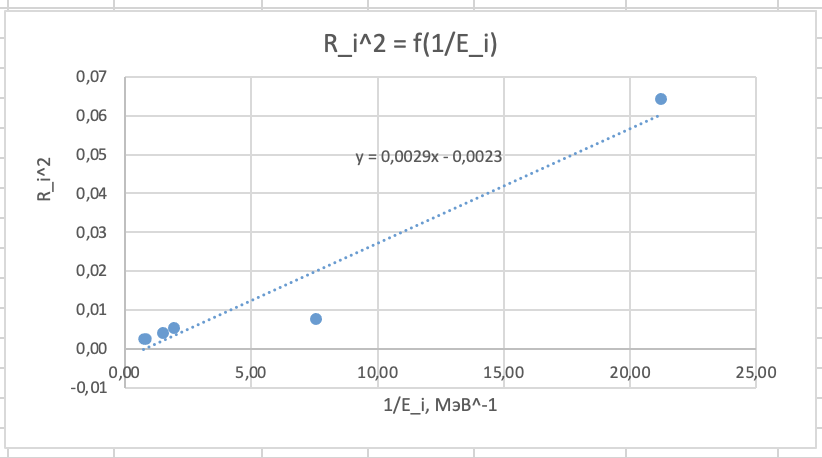
\includegraphics[scale=0.85]{График_3.PNG}
\end{figure}

	\item В спектрах источников, в которых наблюдается энергия фотопиков ($^{22}$Na,  $^{60}$Co,  $^{137}$Cs),  определим энергии фотопиков и сравним эти значения со значениями,  измеренными по формуле $E' = \frac{E}{1 + \frac{2E}{mc^2}}$.

\newpage
	
\begin{figure}[h!]
	\centering
	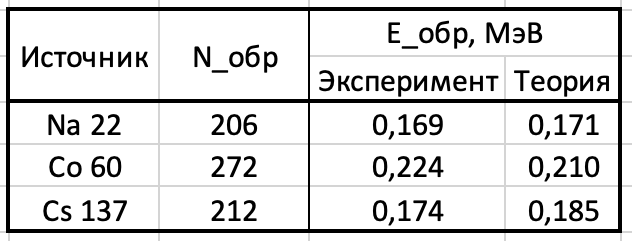
\includegraphics[scale=0.85]{Таблица_3.PNG}
\end{figure}

	\item Построим теоретический график $E_{\text{обр}} = f(E_i)$ и эксперементально полученные точки:

\begin{figure}[h!]
	\centering
	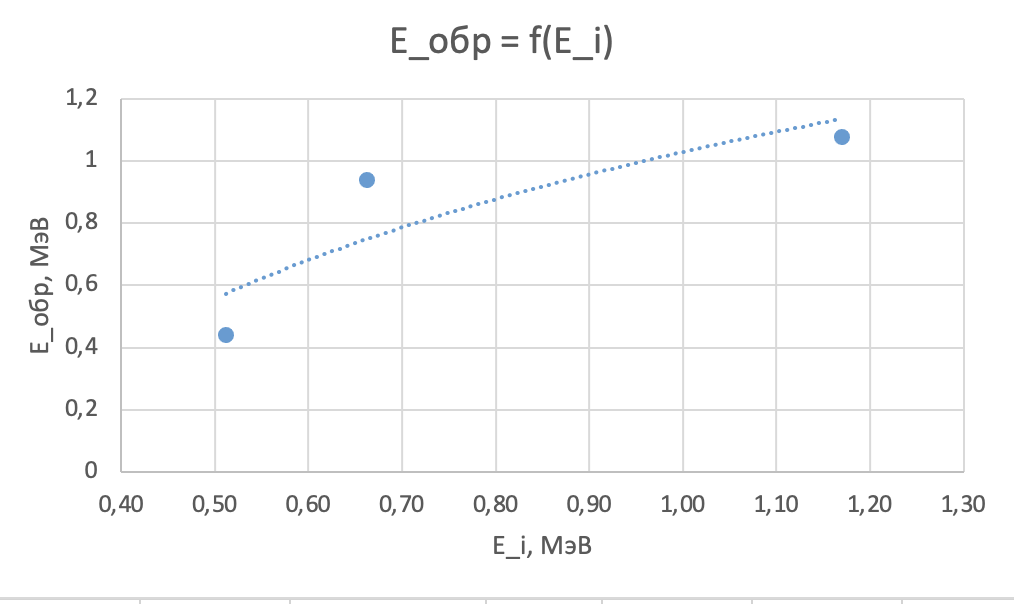
\includegraphics[scale=0.85]{График_4.PNG}
\end{figure}

\end{enumerate}

\textbf{Вывод:}\\\par

В ходе работы сняты спектры образцов $^{22}$Na,  $^{60}$Cо,  $^{137}$Cs, $^{241}$Am, $^{152}$Eu.  Были исследованы пики, соответствующие следующим взаимодействиям гамма-квантов с веществом: фотоэффект, эффект Комптона.  Также была проверена линейная зависимость квадрата спектрального разрешения прибора от величины, обратной энергии полного поглощения.

\end{document}